\documentclass{article}

\title{Assigment3 - Suffix Tree \& Whole genome alignment}
\date{\today}
\author{Weize Xu}

\usepackage{sectsty}
\sectionfont{\fontsize{12}{12}\selectfont}

\usepackage{geometry}
\geometry{
    a4paper,
    total={170mm,257mm},
    left=30mm,
    right=20mm,
    top=20mm,
    }

\renewcommand{\baselinestretch}{1.2}

\usepackage[linesnumbered,boxed,lined]{algorithm2e}

\usepackage{graphicx}
\usepackage{subcaption}

\usepackage{hyperref}
\hypersetup{
    colorlinks=true,
    linkcolor=blue,
    filecolor=magenta,      
    urlcolor=cyan,
}

\usepackage{listings}


\begin{document}

\maketitle

\section{Please give the generalized suffix tree for $S_1$=$ACGT\$$ and $S_2$=$TGCA\#$.}

\large{\textbf{Answer:}}

See Fig.\ref{fig:q1}. (My code for building and visualizing suffix tree, see: 
\url{https://github.com/Nanguage/suffix-trees})

\begin{figure}[h]
    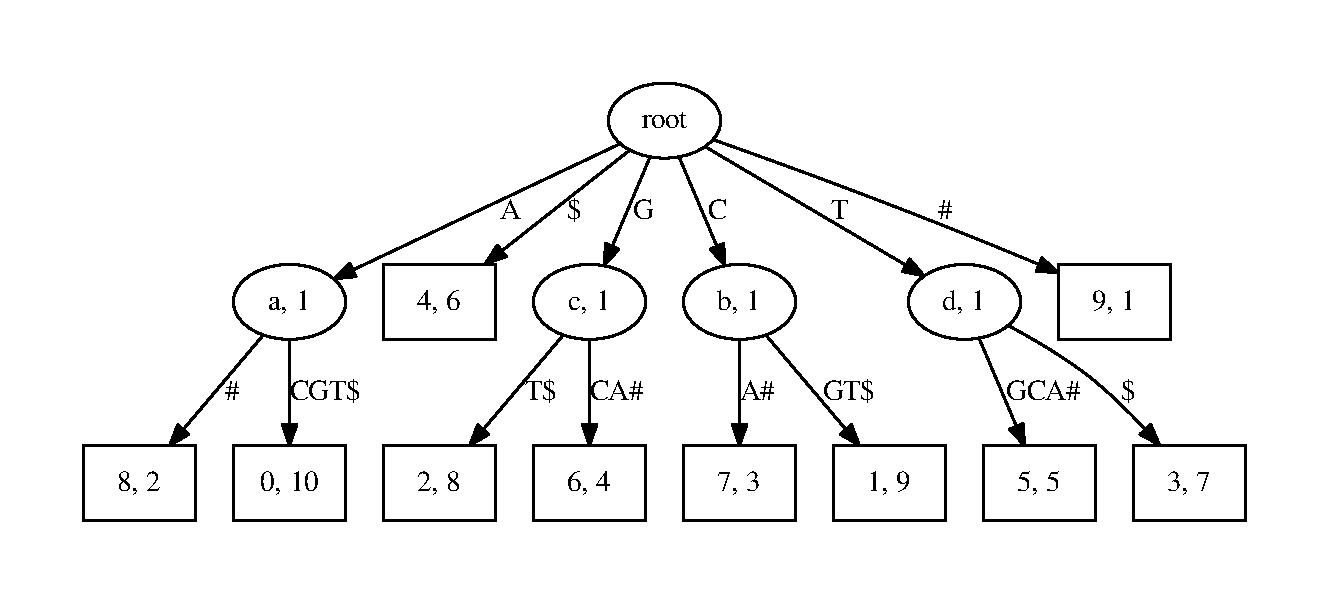
\includegraphics[width=\linewidth]{./img/q1.pdf}
    \caption{Generalized suffix tree.}
    \label{fig:q1}
\end{figure}

\section{Consider a reference genome $T[1..n]$ and a read $R[1..m]$ where $n > m$. We
want to report all positions $i$ such that $Hamming(R, T[i..i+m-1]) \leq k$. Please
propose an $O(kn)$ - time algorithm. (Hint: We can build the suffix tree for
$T\#R\$$ and the corresponding longest common prefix data structure using 
$O(n+m)$ time.)}

\large{\textbf{Answer:}}

\section{Consider $S_1$=$AAAACGTCGGGATCG$ and $S_2$=$GGGCGTAAAGCTCT$.
Suppose the minimum length of MUM is 3. \\
(a) What is the set of MUMs? \\
(b) If we further require that the MUMs are also unique in the sequence
and its reverse complement, what is the set of MUMs?
}

\large{\textbf{Answer:}}

(a): The set of MUMs is $\{CGT, GGG\}$

(b): If consider unique in the reverse complement sequence, the set of MUMs is:
$\{GGG, CCC\}$

\section{Let $A$=$1 2 3 ... 9$ and $B$=$9 6 1 4 7 2 3 5 8$. Suppose we run the $O(n log(n))$ -
time algorithm to find the longest common subsequence. Can you report the
list of tuples stored in $T_i$ for $i$=$0, 1, ..., 9$? Please discuss how do you construct
$T_i$ from $T_{i-1}$.
}

\large{\textbf{Answer:}} \\

\begin{tabular}{l|l}
    \hline
    t & Tuples \\
    \hline
    1 & \{(2, 1)\}\\
    2 & \{(2, 1), (5, 2)\}\\
    3 & \{(2, 1), (5, 2), (6, 3)\}\\
    4 & \{(2, 1), (3, 2), (6, 3)\}\\
    5 & \{(2, 1), (3, 2), (6, 3), (7, 4)\}\\
    6 & \{(1, 1), (3, 2), (6, 3), (7, 4)\}\\
    7 & \{(1, 1), (3, 2), (4, 3), (7, 4)\}\\
    8 & \{(1, 1), (3, 2), (4, 3), (7, 4), (8, 5)\} \\
    9 & \{(0, 1), (3, 2), (4, 3), (7, 4), (8, 5)\}
\end{tabular} \\

Construct $T_i$ from $T_{i-1}$:
\begin{enumerate}
    \item Delete all tuples ($j$, $C_{i-1}[j]$) where $j \geq \delta(i)$ and $C_{i-1} \leq C{i-1}[\delta(i) - 1] + 1$
    \item Insert $(\delta(i), C_{i-1}[\delta(i)-1]+1)$
\end{enumerate}

Implementation see \\
\url{https://github.com/Nanguage/Course-Algorithms-in-Bioinformatics/blob/master/L09/bs_lcs.py}.

\end{document}